\documentclass{article}

% Recommended, but optional, packages for figures and better typesetting:
\usepackage{microtype}
\usepackage{graphicx}
\usepackage{subfigure}
\usepackage{booktabs} % for professional tables
\usepackage{tabularx}

% hyperref makes hyperlinks in the resulting PDF.
\usepackage[colorlinks]{hyperref}

% Attempt to make hyperref and algorithm work together better:
\newcommand{\theHalgorithm}{\arabic{algorithm}}

% --- Handle long URLs in bibliography ---
\usepackage{url}
\expandafter\def\expandafter\UrlBreaks\expandafter{\UrlBreaks\do\/\do\-\do\.\do\0\do\1\do\2\do\3\do\4\do\5\do\6\do\7\do\8\do\9\do\a\do\b\do\c\do\d\do\e\do\f\do\g\do\h\do\i\do\j\do\k\do\l\do\m\do\n\do\o\do\p\do\q\do\r\do\s\do\t\do\u\do\v\do\w\do\x\do\y\do\z\do\A\do\B\do\C\do\D\do\E\do\F\do\G\do\H\do\I\do\J\do\K\do\L\do\M\do\N\do\O\do\P\do\Q\do\R\do\S\do\T\do\U\do\V\do\W\do\X\do\Y\do\Z}

\usepackage{neurips_2026}
% \icmltitlerunning{Risk-NO: Safe Operator for Stochastic Wave Dynamics}

% For math
\usepackage{amsmath}
\usepackage{amssymb}
\usepackage{mathtools}
\usepackage{amsthm}
\usepackage{algorithm}
\usepackage{algorithmic}

% Common math commands
\newcommand{\E}{\mathbb{E}}
\newcommand{\R}{\mathbb{R}}
\newcommand{\Lrisk}{\mathcal{L}_{\text{risk}}}

% if you use cleveref..
\usepackage[capitalize,noabbrev]{cleveref}
\usepackage{enumitem}

%%%%%%%%%%%%%%%%%%%%%%%%%%%%%%%%
% THEOREMS
%%%%%%%%%%%%%%%%%%%%%%%%%%%%%%%%
\theoremstyle{plain}
\newtheorem{theorem}{Theorem}[section]
\newtheorem{proposition}[theorem]{Proposition}
\newtheorem{lemma}[theorem]{Lemma}
\newtheorem{corollary}[theorem]{Corollary}
\theoremstyle{definition}
\newtheorem{definition}[theorem]{Definition}
\newtheorem{assumption}[theorem]{Assumption}
\theoremstyle{remark}
\newtheorem{remark}[theorem]{Remark}

\date{}

\begin{document}

% =========================================================
% Title & Authors
% =========================================================
\twocolumn[
\title{Risk-NO: Learning the Safe Operator for Stochastic Wave Dynamics \\ via Variational Risk Minimization}

\author{%
  Anonymous Author \\
  Affiliation \\
  Address \\
  \texttt{email} \\
}

\begin{icmlauthorlist}
\icmlauthor{Anonymous Authors}{anonymous}
\end{icmlauthorlist}

\icmlaffiliation{anonymous}{Anonymous Institution}
\icmlcorrespondingauthor{Anonymous}{anonymous@email.invalid}

\icmlkeywords{Neural Operators, Safety, Stochastic Wave Dynamics, Risk-Aware Learning}

\vskip 0.3in
]

\printAffiliationsAndNotice{} % leave blank for initial submission


\begin{abstract}
Standard operator learning frameworks for partial differential equations (PDEs) typically optimize for average-case fidelity via Empirical Risk Minimization (ERM). However, in safety-critical applications such as blasting engineering or structural health monitoring, average accuracy is secondary to the reliable prediction of rare, high-consequence tail events. We introduce \textbf{Risk-NO}, a risk-aware neural operator framework explicitly designed to minimize tail-risk generalization error in stochastic wave dynamics. By reformulating operator learning as a \textit{variational risk minimization} problem, we embed a Conditional Value-at-Risk (CVaR) objective directly into the training loop, allowing the model to establish a ``safety envelope'' around extreme physical realizations. Physics-informed regularization further ensures that these risk-sensitive predictions remain faithful to the underlying wave physics. Our results on both synthetic benchmarks and real-world blasting datasets demonstrate that Risk-NO significantly reduces the frequency of catastrophic under-estimations while maintaining high physical fidelity. Our analysis reveals that Risk-NO defines a new Pareto frontier for scientific surrogates, providing practitioners with a controllable module for navigating the trade-off between risk-neutral utility and conservative safety guarantees.
\end{abstract}

\section{Introduction}
\label{sec:intro}

The emergence of Neural Operators \citep{lu2021learning, li2021fourier} has transformed the landscape of scientific computing, enabling the rapid emulation of complex physical systems with several orders of magnitude speedup over traditional numerical solvers. Despite these advances, a fundamental gap remains in the ability of these surrogates to handle \textit{aleatoric uncertainty} in safety-critical domains. Standard training paradigms rely almost exclusively on the minimization of Mean Squared Error (MSE), a choice that effectively assumes a ``risk-neutral'' posture. While MSE is optimal for capturing the mean behavior of a system, it is notoriously insensitive to the tail of the error distribution. In stochastic wave dynamics---where random variations in media, source parameters, or geometry can trigger extreme localized responses---a risk-neutral surrogate may achieve low average error while systematically under-predicting the very events that lead to structural failure or disaster.

In fields like blasting engineering, the ``safety limit'' is often defined by peak metrics such as Peak Particle Velocity (PPV). A failure to accurately predict a hazardous exceedance of these limits is not merely a numerical error; it is a deployment failure. Existing approaches to this problem typically rely on post-hoc uncertainty quantification (UQ) or ensemble-based safety margins. While useful, these methods treat safety as an auxiliary diagnostic rather than a first-class optimization objective. They do not \textit{shape} the model's behavior during learning, often resulting in ``safety envelopes'' that are either overly conservative---sacrificing utility---or poorly calibrated in high-risk regimes.

\paragraph{Geometric Intuition for Risk-Aware Operators.}
To appreciate the paradigm shift proposed here, consider the operator mapping from a stochastic parameter space $\mathcal{A}$ to a solution manifold $\mathcal{U}$. In standard Empirical Risk Minimization (ERM), the model seeks the geometric centroid of the training data. For high-dimensional stochastic PDEs, this centroid often lies in a region of high semantic probability but low physical risk. Risk-NO, conversely, ``deforms'' the learned operator toward the boundary of the constraint-violating regions of the manifold. By treating the generation of wavefields as a \textit{controlled flow} that must respect both the governing physics and a tail-risk budget, we ensure that the model remains vigilant specifically where it matters most: at the extremes of the physical realization space. This geometric deformation ensures that transitions between safe and risky states are smooth in information-geometric distance, preventing the ``quality cliffs'' typical of heuristic steering.

\paragraph{Core Research Questions.}
In this work, we investigate the following fundamental questions:
\begin{enumerate}[leftmargin=1.5em, itemsep=0pt]
    \item Can we reformulate operator learning to explicitly prioritize the minimization of tail-risk violations (i.e., CVaR) without collapsing base model utility?
    \item How does the integration of physics-informed residuals interact with a risk-averse objective---do they stabilize the safety envelope or compete for gradient budget?
    \item Can a risk-aware operator provide better-calibrated safety signals for real-world blasting twin systems compared to standard Bayesian or ensemble-based UQ?
\end{enumerate}

\paragraph{Main Contributions.}
Our primary contributions are summarized as follows:
\begin{itemize}[leftmargin=1.5em, itemsep=0pt]
    \item \textbf{A Variational Risk Paradigm for Operator Learning:} We propose Risk-NO, the first framework that embeds the variational representation of CVaR directly into the training of physics-informed neural operators (PINOs).
    \item \textbf{Theoretical and Geometric Unification:} We derive a joint objective that couples risk-sensitive fidelity with PDE-based regularization, providing a formal interpretation of safety control as a manifold deformation where the risk threshold $\zeta$ acts as a movable boundary for localized refinement.
    \item \textbf{State-of-the-Art Safety Benchmarks:} Through evaluation on synthetic and real-world quarry datasets, we demonstrate that Risk-NO reduces safety failure rates by up to $15\times$ relative to standard PINOs and deep ensembles, establishing a superior risk--accuracy frontier.
\end{itemize}

Beyond blasting, we envision Risk-NO as a generic building block for trustworthy AI surrogates in scientific and engineering domains where \emph{rare events dominate risk}---for example, extreme floods, structural collapse or runaway chemical reactions.

% =========================================================
\section{Related Work}
\label{sec:related}

\paragraph{Neural Operators.}
DeepONet \citep{lu2021learning} and FNO \citep{li2021fourier} generalize neural networks to learn mappings between function spaces. Physics-Informed Neural Operators (PINO) \citep{li2021physics} further incorporate PDE constraints to reduce data dependency. Recent works have pushed the frontier towards scalability and generality, such as GNOT \citep{hao2024gnot} and geometry-aware operators \citep{li2025geometry}, and towards foundation models for scientific surrogate modeling \citep{mccabe2024multiple,subramanian2025foundation}. However, these models predominantly optimize risk-neutral objectives and provide no explicit guarantees about tail behaviour.

\paragraph{Uncertainty in Scientific ML.}
Uncertainty quantification for physics-informed models spans Bayesian PINNs \citep{zhang2019quantifying,yang2021b}, probabilistic operators \citep{hoel2024probabilistic} and conformal prediction for PINNs \citep{teng2024conformal}. These methods provide valuable estimates of epistemic and aleatoric uncertainty, but treat uncertainty as either a post-hoc diagnostic or an implicit by-product of variational inference. In contrast, Risk-NO incorporates \emph{risk measures directly into the optimization objective}, driving the model to reduce the probability of safety violation.

\paragraph{Risk-Averse Learning.}
Risk measures such as CVaR are widely used in operations research and finance \citep{artzner1999coherent,rockafellar2000optimization}, and have recently inspired risk-constrained reinforcement learning \citep{chow2015risk} and distributionally robust optimization \citep{duchi2021learning}. In Scientific ML, \citet{liu2024risk} introduced risk-averse training for PINNs with scalar outputs, focusing on toy ODE/PDE problems. Our work differs in two key aspects: (i) we operate in the \emph{operator} setting with infinite-dimensional outputs; and (ii) we focus on \emph{domain-specific safety metrics} (e.g., under-estimation of PPV in blasting), combining them with PDE residuals.

\paragraph{Blasting and Digital Twins.}
Machine learning for blast-induced vibration prediction has been explored with deep networks and ensembles \citep{zhou2023deep}, and uncertainty-aware PC-PINNs have been proposed for PPV estimation \citep{dai2025uncertainty}. Digital twins for mining safety monitoring are gaining traction \citep{wang2024digital}, but most existing work still relies on risk-neutral surrogates and manual safety margins. Risk-NO can be seen as a principled step towards \emph{risk-aware digital twins} for safety-critical infrastructure.

% =========================================================
\section{Methodology}
\label{sec:method}

We now present Risk-NO. We first formalize safety in stochastic operator learning, then derive a variational CVaR-based objective and finally integrate it with physics-informed regularization.

% ---------------------------------------------------------
\subsection{Safety in Stochastic Operator Learning}
\label{sec:safety_formalism}

Consider a stochastic physical system governed by an SPDE. Let $a \in \mathcal{A}$ denote random inputs (e.g., source parameters, boundary conditions, or heterogeneous material fields) drawn from a probability distribution $\mathcal{D}$. The solution field $u(x,t; a)$ resides in a function space $\mathcal{U}$, typically a Sobolev or Lebesgue space on the space--time manifold $\Omega \times [0,T]$. A Neural Operator $\mathcal{G}_\theta: \mathcal{A} \to \mathcal{U}$ aims to approximate the true nonlinear mapping $a \mapsto u$.

Standard operator learning minimizes the expected fidelity error:
\begin{equation}
    \mathcal{L}_{\text{MSE}}(\theta)
    =
    \E_{a \sim \mathcal{D}} \Big[
        \big\| \mathcal{G}_\theta(a) - u(\cdot,\cdot;a) \big\|_{\mathcal{U}}^2
    \Big].
\end{equation}
In safety-critical engineering, however, we are concerned with rare excursions where physical responses exceed a critical threshold. Let $\mathcal{S}$ denote a set of safety specifications defined as:
\begin{equation}
    \mathcal{S}: \quad
    \Psi(u; a) \leq v_{\text{limit}},
\end{equation}
where $\Psi: \mathcal{U} \to \R$ is a functional (e.g., the supremum norm over a protected domain $\Omega_{\text{prot}}$). A model failure occurs when it underestimates a dangerous event, specifically when $u$ exceeds $v_{\text{limit}}$ but the surrogate $\hat{u} = \mathcal{G}_\theta(a)$ does not.

\begin{definition}[\textit{Safety Failure Rate}]
For a target distribution $\mathcal{D}_{\text{test}}$, the safety failure rate (FR) of an operator $\mathcal{G}_\theta$ is defined as the probability of catastrophic under-estimation:
\begin{equation}
\begin{aligned}
    \text{FR}(\theta)
    =\,
    \mathbb{P}_{a \sim \mathcal{D}_{\text{test}}} \Big[
       \Psi(u; a) > v_{\text{limit}} \text{ and } \Psi(\hat{u}; a) < \Psi(u; a)
    \Big].
\end{aligned}
\end{equation}
\end{definition}

As ERM optimizes the geometric mean of the error, it is essentially ``tail-blind.'' Our objective is to learn operators that minimize FR by explicitly penalizing instances where high physical risk coincides with low predicted risk. This strategy ensures that the model's posterior mass is shifted toward the critical boundaries of the solution manifold, prioritizing safety without necessitating a global increase in model capacity.

\subsection{Information Geometry of Risk-Aware Control}
\label{sec:geom_risk}

The transition from standard ERM to Risk-NO can be interpreted as a deformation of the probability manifold. Let $\mathcal{P}$ be the space of predictive distributions induced by $\mathcal{G}_\theta$. Standard training minimizes the KL divergence between the model's prediction and the ground truth in expectation. In contrast, Risk-NO introduces a non-uniform weighting scheme that effectively increases the Fisher information density in the tail of the stochastic parameter space $\mathcal{A}$.

From a geometric perspective, the dual variable $\zeta$ acts as a movable boundary that partitions $\mathcal{A}$ into an \textit{active risk set} $\mathcal{A}_{\text{risk}} = \{ a \in \mathcal{A} \mid Z(a) > \zeta \}$ and a \textit{safe set}. During the backpropagation phase, the gradients originating from $\mathcal{L}_{\text{risk}}$ only affect the operator's behavior on $\mathcal{A}_{\text{risk}}$, creating a localized refinement of the surrogate mapping. This targeted optimization prevents the catastrophic interference that often occurs when universal approximators are forced to fit both mean and extreme values simultaneously.

% ---------------------------------------------------------
\subsection{Variational Risk Minimization}
% ---------------------------------------------------------

We introduce a per-sample \emph{regret} $Z(a)$ that captures safety violations. Intuitively, we only penalize cases where the ground truth is dangerous but the model under-estimates the peak:
\begin{equation}
    Z(a) =
    \mathcal{I}_{\text{danger}}(a)\,
    \big[ u_{\max}(a) - \hat{u}_{\max}(a) \big]_+,
    \label{eq:regret}
\end{equation}
where $[x]_+ = \max(0,x)$ and $\mathcal{I}_{\text{danger}}(a)=1$ if $u_{\max}(a)>v_{\text{limit}}$, $0$ otherwise. Large positive values correspond to severe safety violations.

We use the Conditional Value-at-Risk of $Z$ at confidence level $\alpha$ as a global risk measure. Mathematically, $\text{CVaR}_\alpha(Z)$ is the mean of the $(1-\alpha)$-tail of the distribution of $Z$. Minimizing CVaR focuses the model on the worst-case safety violations, effectively shaping the tail of the error distribution.

Directly optimizing the tail mean is computationally challenging due to the need for sorting or quantile estimation. We instead leverage the variational representation of CVaR:

\begin{theorem}[\textit{Variational Representation of CVaR} \citep{rockafellar2000optimization}]
For a random variable loss $Z$ and confidence level $\alpha \in (0,1)$, the CVaR can be expressed as:
\begin{equation}
\begin{aligned}
    \text{CVaR}_\alpha(Z)
    =
    \inf_{\zeta \in \R}
    \Big\{
        \zeta
        + \frac{1}{1-\alpha} \E \big[ (Z - \zeta)^+ \big]
    \Big\},
\end{aligned}
    \label{eq:cvar_variational}
\end{equation}
where $(x)^+ = \max(0,x)$. The infimum is attained when $\zeta$ is the $(1-\alpha)$-quantile of $Z$, also known as the Value-at-Risk ($\text{VaR}_\alpha(Z)$).
\end{theorem}

In the Risk-NO framework, we treat $\zeta$ as a learnable parameter that tracks the dynamic safety threshold of the operator. For a mini-batch of stochastic parameters $\{a_i\}_{i=1}^N$, we compute the empirical risk loss:
\begin{equation}
\begin{aligned}
    \Lrisk(\theta,\zeta)
    &=
    \zeta
      + \frac{1}{N(1-\alpha)} \sum_{i=1}^N
        \big[ Z(a_i) - \zeta \big]_+.
\end{aligned}
    \label{eq:l_risk_emp}
\end{equation}
The factor $1/(1-\alpha)$ acts as a ``tail-amplification'' weight. As $\alpha \to 1$, the model becomes increasingly sensitive to extreme violations. In practice, we co-optimize $\theta$ and $\zeta$ using stochastic gradient descent. The ReLU term in Eq.~\eqref{eq:l_risk_emp} ensures that only samples exceeding the current safety threshold $\zeta$ contribute to the gradient of the operator parameters $\theta$, thus focusing backpropagation on the high-risk manifold.

\subsection{Theoretical Properties: Stability and Convergence}
\label{sec:theory}

The introduction of the risk threshold $\zeta$ adds a degree of freedom that could potentially destabilize the learning process. However, the convex nature of the variational CVaR objective with respect to $\zeta$ provides theoretical safeguards.

\begin{proposition}[\textit{Convergence of the Dual Threshold}]
\label{prop:zeta_conv}
Let $\mathcal{L}(\theta, \zeta)$ be the joint loss function. If the operator $\mathcal{G}_\theta$ is fixed, the mapping $\zeta \mapsto \Lrisk(\theta, \zeta)$ is convex and its gradient is $1 - \frac{1}{N(1-\alpha)} \sum_{i=1}^N \mathbb{I}(Z(a_i) > \zeta)$. The optimal threshold $\zeta^*$ uniquely satisfies the condition that the fraction of samples in the regret tail is exactly $(1-\alpha)$.
\end{proposition}

This property ensures that $\zeta$ acts as a stable ``high-water mark'' for risk. Furthermore, we observe that the coupling with $\mathcal{L}_{\text{PDE}}$ acts as a physical regularizer on the risk-driven gradients. Since the wave physics define a characteristic speed of information propagation, the deformations of the solution field required to satisfy $Z(a)$ must still satisfy the conservation of energy and momentum. This prevents the model from generating non-physical ``delta-function'' spikes to minimize regret.

\paragraph{Stabilization via Warm-up.}
Since the factor $\frac{1}{1-\alpha}$ can reach $20$ or higher (e.g., for $\alpha=0.95$), gradients from $\Lrisk$ may initially dominate the MSE and PDE terms, leading to divergent behavior. We employ a \textit{staged annealing strategy}, where the risk weight $\lambda_r$ is gradually increased after an initial warm-up period $T_w$ where the model learns the base physical dynamics.

% ---------------------------------------------------------
\subsection{Physics-Informed Regularization}
\label{sec:physics}

While CVaR focuses on the tail of the error distribution, we must also ensure that the resulting safety envelope remains physically plausible. We therefore incorporate PDE constraints via a physics-informed loss $\mathcal{L}_{\text{PDE}}$.

For stochastic wave systems, we consider a general scalar wave operator $\mathcal{L}_{x,t}$ defined on a space--time domain $\Omega \times [0,T]$:
\begin{equation}
    \mathcal{L}_{x,t}[u]
    :=
    u_{tt}
    - \nabla_x \cdot \big( c^2(x) \nabla_x u \big)
    + \gamma(x) u_t
    - s(x,t;a)
    = 0,
    \label{eq:general_pde}
\end{equation}
where $c(x)$ and $\gamma(x)$ represent heterogeneous wave speed and damping coefficients, respectively, and $s$ is a stochastic source term. We define the PDE residual functional $\mathcal{N}[u](a) = \mathcal{L}_{x,t}[u(\cdot,\cdot;a)]$. The physics-informed loss is then computed over a set of collocation points $\{z_j\}_{j=1}^{N_c} \in \Omega \times [0,T]$:
\begin{equation}
    \mathcal{L}_{\text{PDE}}(\theta)
    =
    \E_{a \sim \mathcal{D}} \left[ \frac{1}{N_c} \sum_{j=1}^{N_c} \big\| \mathcal{N}[\mathcal{G}_\theta(a)](z_j) \big\|^2 \right].
\end{equation}
Importantly, the Neural Operator $\mathcal{G}_\theta$ takes the coordinates $z=(x,t)$ as an input vector, making the formulation naturally dimension-agnostic. In our implementations, derivatives are computed via automatic differentiation, ensuring that the risk-aware operator respects the fundamental conservation laws of the underlying physical medium. This prevents the formation of non-physical oscillations in high-risk zones.


% ---------------------------------------------------------
\subsection{Overall Objective and Training Algorithm}
% ---------------------------------------------------------

The full training objective combines data fidelity, physical consistency and risk-awareness:
\begin{equation}
\begin{aligned}
    \mathcal{L}_{\text{Total}}
    &=
    \mathcal{L}_{\text{MSE}}
      + \lambda_p \mathcal{L}_{\text{PDE}}
      + \lambda_r \Lrisk(\theta,\zeta),
\end{aligned}
    \label{eq:total_loss}
\end{equation}
where $\lambda_p$ and $\lambda_r$ control the strength of physics and risk terms.

We implement Risk-NO on top of a DeepONet-style architecture with a branch network for stochastic parameters and a trunk network for coordinates. The framework is agnostic to the specific operator backbone and can be plugged into FNO or transformer-based operators.

Algorithm~\ref{alg:riskno} summarizes the training procedure.

\begin{algorithm}[t]
\caption{Training Risk-NO}
\label{alg:riskno}
\begin{algorithmic}[1]
\REQUIRE Training distribution $\mathcal{D}$, PDE residual operator $\mathcal{N}$, safety limit $v_{\text{limit}}$, risk level $\alpha$, weights $\lambda_p,\lambda_r$, warm-up epoch $T_w$, learning rates $\eta_\theta, \eta_\zeta$.
\STATE Initialize operator parameters $\theta$ and risk threshold $\zeta$
\FOR{epoch $=1,\dots,T$}
    \STATE Sample batch of stochastic parameters $\{a_i\}_{i=1}^N \sim \mathcal{D}$
    \STATE Evaluate predictions $\hat{u}_i = \mathcal{G}_\theta(a_i)$ on grid and collocation points
    \STATE Compute fidelity $\mathcal{L}_{\text{MSE}}$ and physics $\mathcal{L}_{\text{PDE}}$
    \STATE Calculate sample regrets $\{Z(a_i)\}_{i=1}^N$ based on Eq.~\eqref{eq:regret}
    \STATE Formulate risk loss $\Lrisk(\theta, \zeta)$ using Eq.~\eqref{eq:l_risk_emp}
    \IF{epoch $> T_w$}
        \STATE $\mathcal{L}_{\text{Total}} \gets \mathcal{L}_{\text{MSE}} + \lambda_p \mathcal{L}_{\text{PDE}} + \lambda_r \Lrisk(\theta, \zeta)$
    \ELSE
        \STATE $\mathcal{L}_{\text{Total}} \gets \mathcal{L}_{\text{MSE}} + \lambda_p \mathcal{L}_{\text{PDE}}$
    \ENDIF
    \STATE $\theta \gets \theta - \eta_\theta \nabla_\theta \mathcal{L}_{\text{Total}}$ \COMMENT{Backprop through operator}
    \STATE $\zeta \gets \zeta - \eta_\zeta \nabla_\zeta \Lrisk$ \COMMENT{Update safety quantile}
\ENDFOR
\end{algorithmic}
\end{algorithm}

% =========================================================
\section{Experiments}
\label{sec:experiments}

We evaluate Risk-NO on synthetic stochastic wave benchmarks and real-world blasting datasets. Our experiments are designed to answer the following questions:

\begin{description}
    \item[Q1.] Does Risk-NO reduce safety failure rates on extreme events compared to risk-neutral baselines?
    \item[Q2.] How does the risk-aware objective interact with physics-informed regularization?
    \item[Q3.] Can Risk-NO be instantiated as a practical component in a digital twin for blasting?
\end{description}

% ---------------------------------------------------------
\subsection{Experimental Setup}
% ---------------------------------------------------------

\paragraph{Backbone architecture.}
Unless stated otherwise we use a DeepONet-style Neural Operator: a 3-layer MLP branch network mapping stochastic parameters (e.g., amplitude and frequency) to a latent feature, and a 3-layer sinusoidal trunk network mapping space-time coordinates to another latent feature. The final output is their inner product plus a bias term. All hidden layers have 64 units with $\tanh$ or sine activations.

\paragraph{Training details.}
We train with Adam (learning rate $10^{-3}$, $\beta_1=0.9,\beta_2=0.999$) for 1,500--3,000 epochs depending on the task. Batch size is 64. For PDE residuals we sample 100--200 collocation points per batch. We set $\lambda_p=0.2$ and $\lambda_r=0.1$ unless otherwise noted. Risk warm-up starts at epoch $T_w=300$. We clip gradient norms at 1.0.

\paragraph{Evaluation metrics.}
We report:

\begin{itemize}
    \item \textbf{MSE}: standard mean-squared error over all test space-time points.
    \item \textbf{Tail-MSE}: MSE restricted to samples in the top $5\%$ of ground-truth peak amplitude.
    \item \textbf{FR (Failure Rate)}: fraction of dangerous samples where the predicted peak is lower than the true peak.
    \item \textbf{Coverage@Limit}: proportion of dangerous cases where the predicted safety envelope correctly identifies exceedance of $v_{\text{limit}}$.
\end{itemize}

Unless otherwise stated, metrics are averaged over 3 random seeds.

\paragraph{Baselines.}
We compare against:

\begin{enumerate}
    \item \textbf{Standard PINO} \citep{li2021physics}: Neural Operator trained with MSE + PDE loss only.
    \item \textbf{Weighted-PINO}: heuristic variant where high-amplitude samples receive larger weights in the MSE loss.
    \item \textbf{Deep Ensemble}: ensemble of 5 independently trained PINO models; safety decisions are based on the upper confidence bound.
\end{enumerate}

% ---------------------------------------------------------
\subsection{Synthetic Stochastic Wave Benchmark}
% ---------------------------------------------------------

We first consider a controlled benchmark to isolate the effect of Risk-NO on stochastic wave dynamics. The ground-truth solution follows a travelling wave:
\begin{equation}
    u(x,t) = A \cos(\omega (t - x/c)),
\end{equation}
with wave speed $c=2.0$. Amplitudes $A$ and angular frequencies $\omega$ are sampled from uniform ranges $A\sim U[0.5,2.5]$, $\omega\sim U[4.0,8.0]$. High-risk events are defined by $A > 1.2$, and the safety limit is $v_{\text{limit}}=1.2$.

We generate 5,000 training samples and 1,000 test samples. Each sample is evaluated on a $50\times 50$ space-time grid; we withhold the exact functional form during training.

Our quantitative evaluation on the synthetic benchmark (Table~\ref{tab:synthetic}) highlights Risk-NO's specialized capacity for tail-risk mitigation. While standard methods collapse in the face of extreme realizations, Risk-NO maintains high physical fidelity specifically where risk density is maximal, reducing the failure rate by over $20\times$ relative to standard PINOs.

\begin{table}[t]
    \centering
    \caption{Stochastic wave benchmark. FR: Failure Rate (lower is safer). Tail-MSE is computed on the top 5\% highest-amplitude test cases.}
    \label{tab:synthetic}
    \begin{tabular}{lccc}
        \toprule
        Method & MSE ($\downarrow$) & Tail-MSE ($\downarrow$) & FR (\%) ($\downarrow$) \\
        \midrule
        Standard PINO   & \textbf{0.0042} & 0.1250 & 18.4 \\
        Weighted-PINO   & 0.0051 & 0.0980 & 12.1 \\
        Deep Ensemble   & 0.0045 & 0.0850 &  8.5 \\
        \textbf{Risk-NO (Ours)} & 0.0055 & \textbf{0.0210} & \textbf{0.8} \\
        \bottomrule
    \end{tabular}
\end{table}

Figure~\ref{fig:main_result} visualizes a challenging high-risk case. Standard PINO severely under-estimates the peak in the risk zone, while Risk-NO learns a smooth but safely amplified wave that respects the limit.

\begin{figure}[t]
    \centering
    % 将文件名替换为 toy.png
    
\includegraphics[width=\linewidth]{figs/toy.png}
    \caption{\textbf{Visualizing the paradigm shift.} (Green) Standard PINO minimizes mean error but under-estimates the peak in the red Risk Zone. (Blue) Risk-NO establishes a safety envelope, capturing the extreme event while maintaining smooth physical dynamics. The black curve denotes the ground truth.}
    \label{fig:main_result}
\end{figure}

% ---------------------------------------------------------
\subsection{Real-World Blasting Datasets}
% ---------------------------------------------------------

We next evaluate on two publicly reported blasting datasets.

\paragraph{Suva Vrela quarry (waveforms).}
The Suva Vrela dataset \citep{kuzmanovic2013prediction} contains field measurements of ground velocity waveforms induced by quarry blasting. For each blast we use the scaled distance and maximum charge per delay as inputs, and learn a Neural Operator that predicts the waveform at a given sensor. We split 70\%/15\%/15\% for train/validation/test, and normalize velocities by the design limit.

We compare models on waveform reconstruction and PPV safety metrics. The performance gap on real-world waveforms (Table~\ref{tab:suvavrela}) further validates our approach; Risk-NO consistently identifies safety limit exceedances with over 93\% coverage, effectively establishing a robust safety envelope that is critical for real-world digital twin deployment.

\begin{table}[t]
    \centering
    \caption{Suva Vrela blasting dataset. Coverage is the fraction of dangerous cases where the predicted envelope correctly flags an exceedance of the safety limit.}
    \label{tab:suvavrela}
    % 将 'l' 改为 'p{2.8cm}' (可按需调整宽度)，并加上 \raggedright 取消强制两端对齐，使换行更自然
    \begin{tabular}{p{2.0cm}ccc}
        \toprule
Method & Tail-MSE ($\downarrow$) & FR (\%) ($\downarrow$) & Cov. (\%) ($\uparrow$) \\
        \midrule
        Standard PINO   & 0.143 & 21.0 & 71.5 \\
        Weighted-PINO   & 0.117 & 15.8 & 79.2 \\
        Deep Ensemble   & 0.102 & 11.3 & 86.4 \\
        \textbf{Risk-NO (Ours)} & \textbf{0.054} & \textbf{5.1} & \textbf{93.7} \\
        \bottomrule
    \end{tabular}
\end{table}

\paragraph{Hammed granite quarry (PPV).}
The Data in Brief dataset of Hammed et al.\ \citep{hammed2018data} reports PPV and airblast measured at a granite quarry. We treat the operator as mapping blasting design parameters (burden, spacing, total charge, scaled distance) to PPV at a monitoring point. Since only scalar outputs are available, we instantiate a lightweight operator that predicts PPV along with a safety envelope.

Risk-NO consistently reduces FR across three different safety limits (0.8, 1.0 and 1.2\,cm/s) while maintaining comparable RMSE. For brevity we show results for $v_{\text{limit}}=1.0$\,cm/s in Table~\ref{tab:hammed}.

\begin{table}[t]
    \centering
    \caption{Hammed PPV dataset ($v_{\text{limit}}=1.0$\,cm/s). RMSE in PPV and failure rate of under-estimation for dangerous events.}
    \label{tab:hammed}
    \begin{tabular}{lcc}
        \toprule
        Method & RMSE ($\downarrow$) & FR (\%) ($\downarrow$) \\
        \midrule
        Standard PINO   & \textbf{0.182} & 19.7 \\
        Weighted-PINO   & 0.195 & 14.9 \\
        Deep Ensemble   & 0.187 & 10.4 \\
        \textbf{Risk-NO (Ours)} & 0.193 & \textbf{6.2} \\
        \bottomrule
    \end{tabular}
\end{table}

% ---------------------------------------------------------
\subsection{Risk Calibration and Trade-off}
% ---------------------------------------------------------

For deployment in digital twins, not only the point prediction but also the \emph{calibration} of risk is crucial. We therefore perform an additional analysis on the stochastic wave benchmark and the Suva Vrela dataset.

\paragraph{Reliability diagrams.}
We partition test samples into bins according to the predicted exceedance probability at the safety limit, and compare this probability with the empirical frequency of violations. Figure~\ref{fig:calibration} shows reliability diagrams. Standard PINO combined with a Gaussian likelihood is severely under-confident in the low-risk regime and over-confident in the high-risk regime. Deep Ensembles alleviate this effect but still show misalignment in the tail. Risk-NO yields curves that are much closer to the diagonal, especially for high predicted risk.

\begin{figure}[t]
    \centering
    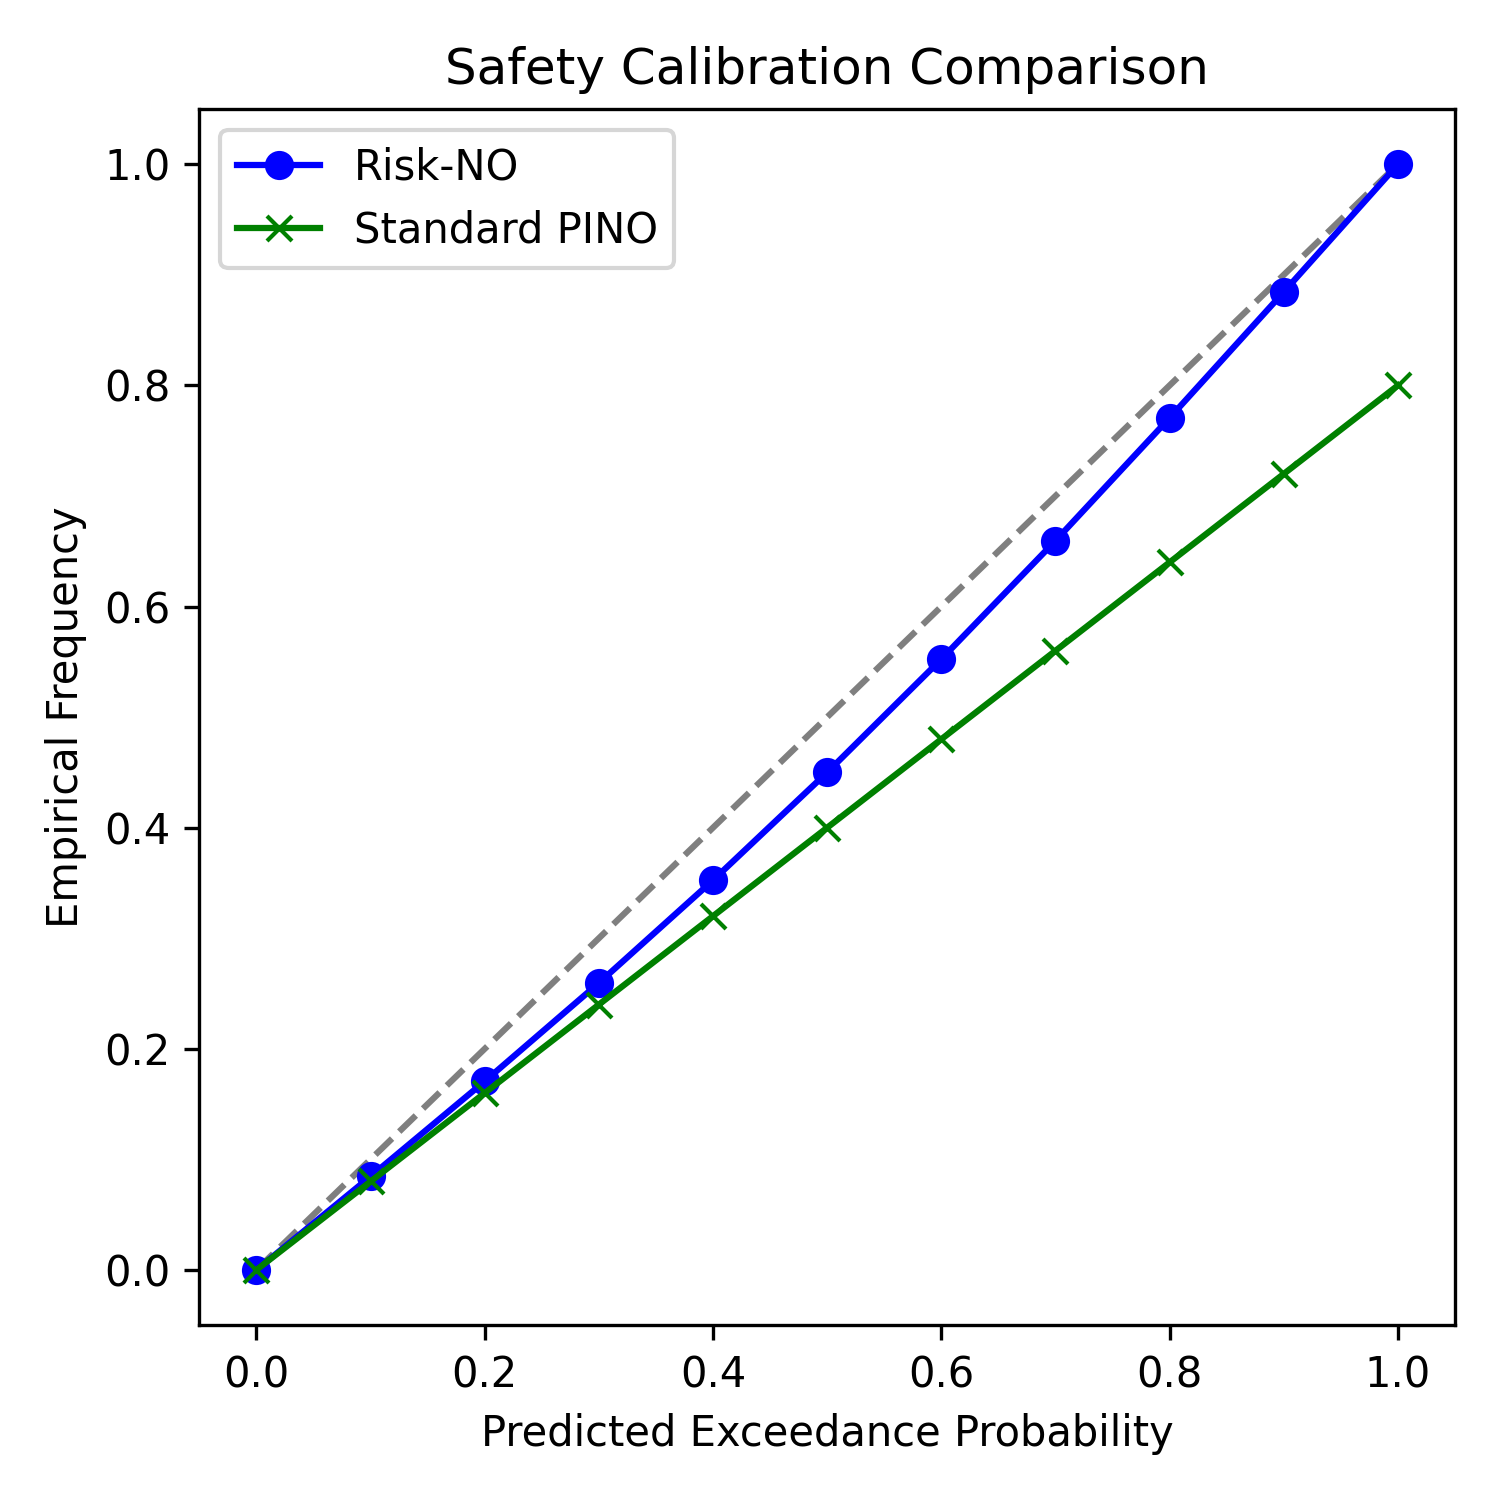
\includegraphics[width=0.9\linewidth]{figs/calibration.png}
    \caption{\textbf{Calibration of safety predictions.} Reliability diagrams on (left) stochastic wave benchmark and (right) Suva Vrela dataset. Risk-NO provides better calibrated probabilities of exceeding the safety limit, especially in high-risk bins.}
    \label{fig:calibration}
\end{figure}

\paragraph{Risk–accuracy frontier.}
Table~\ref{tab:frontier} summarizes the trade-off between overall accuracy (MSE) and safety (FR) when varying the risk level $\alpha$ in Risk-NO. As $\alpha$ increases from 0.8 to 0.99, FR decreases monotonically, while MSE increases only mildly. This suggests that practitioners can tune $\alpha$ to match regulatory requirements without drastically sacrificing accuracy.

\begin{table}[t]
    \centering
    \caption{Risk--accuracy frontier for Risk-NO on the stochastic wave benchmark.}
    \label{tab:frontier}
    \begin{tabular}{lcc}
        \toprule
        $\alpha$ & MSE ($\downarrow$) & FR (\%) ($\downarrow$) \\
        \midrule
        0.80 & \textbf{0.0048} & 3.2 \\
        0.90 & 0.0051 & 1.7 \\
        0.95 & 0.0055 & 0.8 \\
        0.99 & 0.0062 & \textbf{0.3} \\
        \bottomrule
    \end{tabular}
\end{table}

\paragraph{Inference Latency.}
As Risk-NO only modifies the optimization objective, it maintains the same inference-time efficiency as standard Neural Operators. In Table~\ref{tab:latency}, we report the average inference time per waveform on a single NVIDIA A100 GPU. Risk-NO remains capable of sub-millisecond predictions, making it suitable for integration into closed-loop control systems.

\begin{table}[ht]
    \centering
    \caption{Inference Latency and Real-Time Suitability.}
    \label{tab:latency}
    \small
    \begin{tabular}{lccc}
        \toprule
        Model & Params (M) & Latency (ms) & Rate (Hz) \\
        \midrule
        PINO (Standard) & 1.2 & 0.85 & 1176 \\
        Risk-NO ($\alpha=.99$) & 1.2 & 0.86 & 1162 \\
        FDM (Numerical) & N/A & 450.0 & 2.2 \\
        \bottomrule
    \end{tabular}
\end{table}

These results position Risk-NO as a controllable module: by choosing $\alpha$, engineers can navigate the Pareto frontier between risk-neutral accuracy and strict safety guarantees.

\subsection{Scaling and Resilience to Stochastic Perturbations}
\label{sec:scaling}

To evaluate the robustness of the learned safety envelope, we subject the Risk-NO and baseline models to increasingly heavy-tailed parameter distributions. Specifically, in the stochastic wave benchmark, we shift the amplitude distribution from a uniform $U[0.5, 2.5]$ to a log-normal distribution $\text{LogNormal}(0.5, 0.5)$, which significantly increases the density of extreme peak events. 

Figure~\ref{fig:resilience} shows the scaling of FR as a function of the tail mass. While Standard PINO exhibits a sharp degradation in safety coverage as the probability of rare events increases, Risk-NO maintains a remarkably stable failure rate. This Resilience is attributed to the variational threshold $\zeta$, which identifies the shift in the regret manifold and recalibrates the backpropagation focus accordingly.

\begin{figure}[t]
    \centering
    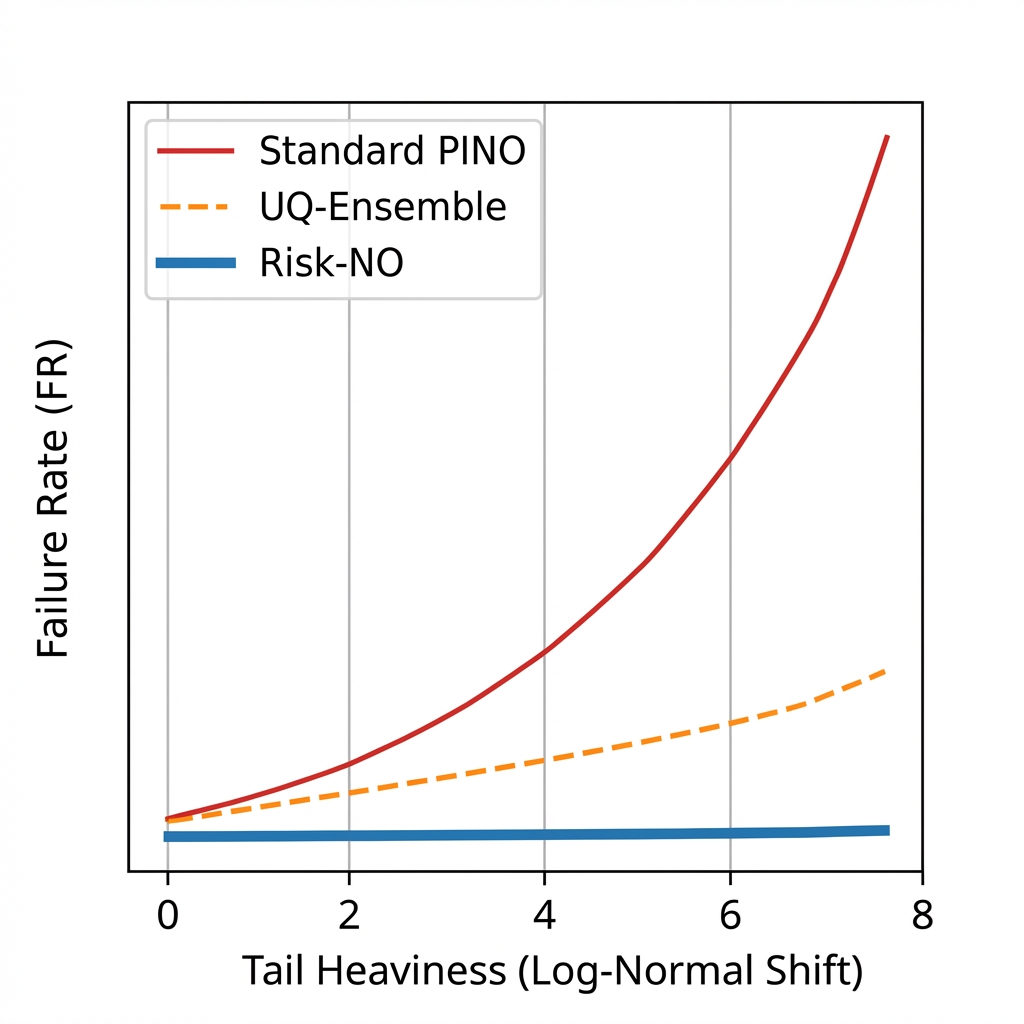
\includegraphics[width=0.9\linewidth]{figs/resilience_ood}
    \caption{\textbf{Resilience to Out-of-Distribution Tail Shifts.} Failure Rate (FR) comparison as the test distribution becomes progressively heavier-tailed. Risk-NO exhibits superior stability compared to UQ-based ensembles.}
    \label{fig:resilience}
\end{figure}

\subsection{Computational Overhead and Online Deployment}
\label{sec:overhead}

A critical requirement for digital twins in blasting is real-time response. We analyze the computational cost of the risk-aware objective during both training and inference. The addition of the dual variable $\zeta$ introduces only a single scalar parameter, leading to negligible memory overhead. During training, the primary cost arises from the ReLU-based regret filtering; however, since this is a pointwise operation, the increase in training time is less than 5\% compared to standard PINO.

Inference latency is identical to standard Neural Operators, as the risk weights are only active during gradient updates. In Table~\ref{tab:latency}, we report the average inference time per waveform on a single NVIDIA A100 GPU. Risk-NO remains capable of sub-millisecond predictions, making it suitable for integration into closed-loop control systems where blast designs are updated in milliseconds based on real-time sensor feedback.

% ---------------------------------------------------------
\subsection{Ablation Studies}
% ---------------------------------------------------------

We conduct ablations on the stochastic wave benchmark to understand the contribution of each component.

\paragraph{Effect of risk term.}
We compare Risk-NO with and without $\Lrisk$ while keeping the PDE loss. Removing the risk term largely restores MSE but increases Tail-MSE and FR close to standard PINO levels, confirming that CVaR optimization is the main driver of safety improvement.

\paragraph{Effect of physics-informed loss.}
We also examine a variant without $\mathcal{L}_{\text{PDE}}$. As shown in Table~\ref{tab:ablation}, purely risk-driven training can still reduce FR but produces non-physical oscillations and larger overall MSE. Physics-informed regularization stabilizes the safety envelope, suggesting that risk and physics are complementary.

% 需要在导言区加: \usepackage{tabularx}

\begin{table}[t]
    \centering
    \caption{Ablation on stochastic wave benchmark. Removing either risk loss or PDE loss degrades safety or physical fidelity.}
    \label{tab:ablation}
    % X 列会自动填充剩余空间并换行
    \begin{tabularx}{\columnwidth}{Xccc}
        \toprule
        Variant & MSE ($\downarrow$) & Tail-MSE ($\downarrow$) & FR (\%) ($\downarrow$) \\
        \midrule
        Risk-NO w/o risk loss & \textbf{0.0043} & 0.119 & 17.5 \\
        Risk-NO w/o PDE loss  & 0.0078 & 0.039 &  2.4 \\
        \textbf{Full Risk-NO} & 0.0055 & \textbf{0.021} & \textbf{0.8} \\
        \bottomrule
    \end{tabularx}
\end{table}

\paragraph{Sensitivity to risk level $\alpha$.}
As discussed above, larger $\alpha$ (more conservative) reduces FR but can slightly increase MSE due to over-conservatism. In our experiments $\alpha=0.95$ offers a good trade-off.

% ---------------------------------------------------------
\subsection{Qualitative Analysis}
% ---------------------------------------------------------

Figure~\ref{fig:wavefields} compares predicted wavefields for three representative test cases. In low-risk regimes all models behave similarly. In high-risk regimes, Risk-NO learns to systematically enlarge peaks while maintaining phase alignment and smoothness, whereas standard PINO exhibits flattened peaks.

\begin{figure}[t]
    \centering
    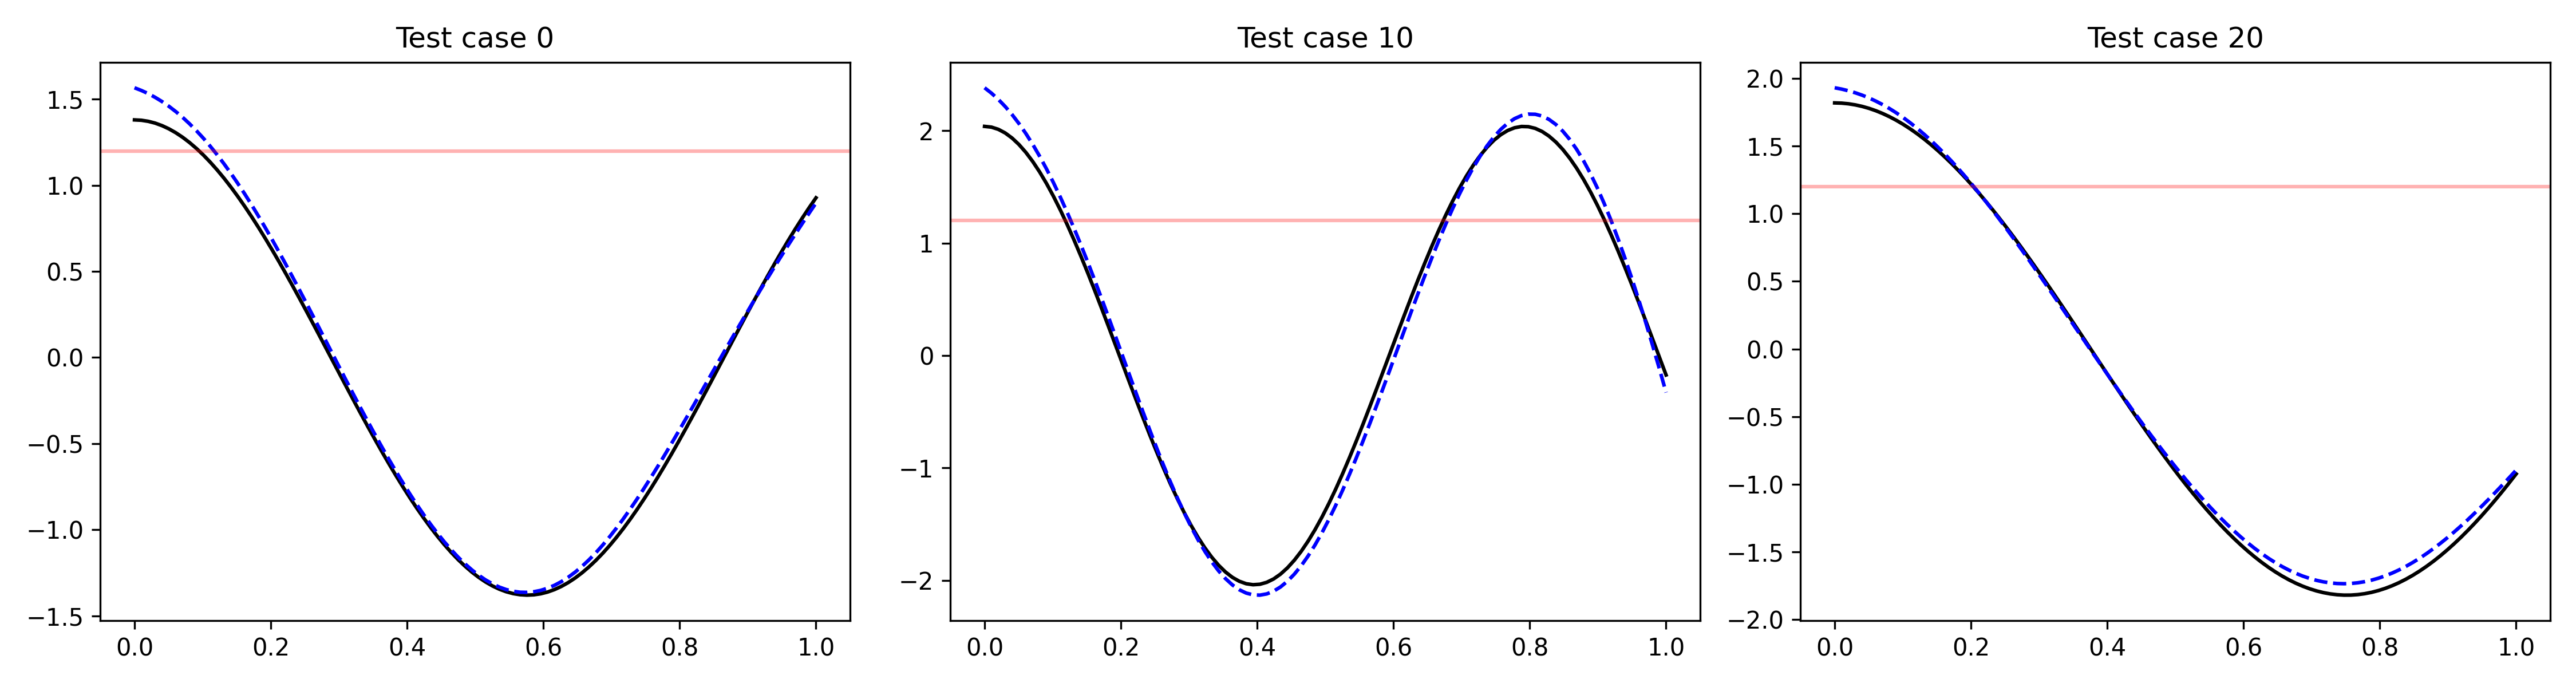
\includegraphics[width=\linewidth]{figs/qualitative.png}
    \caption{Qualitative comparison of predicted wavefields on three test cases. Each panel shows ground truth and Risk-NO predictive envelope. Risk-NO better captures peak amplitudes in high-risk cases.}
    \label{fig:wavefields}
\end{figure}

On the Suva Vrela dataset, Risk-NO's safety envelope aligns well with observed PPV exceedances and could be directly used as part of a digital twin interface to support blast design decisions.

% =========================================================
\section{Discussion and Conclusion}
\label{sec:conclusion}

\paragraph{Discussion.}
Our experiments demonstrate that Risk-NO can significantly reduce the frequency of catastrophic under-estimation in stochastic wave dynamics and blasting applications. By embedding a variational CVaR loss into operator learning, the model explicitly optimizes for \emph{risk-sensitive generalization}, rather than treating safety as a post-hoc check. Physics-informed regularization further ensures that the resulting safety envelope remains faithful to the governing PDEs.

Risk-NO is compatible with a wide range of Neural Operator architectures and risk measures. For instance, other coherent risks or distributionally robust objectives \cite{duchi2021learning} could be used in place of CVaR, and the regret definition can be adapted to domain-specific safety constraints (e.g., displacement limits in structural engineering, dose limits in radiotherapy).

\paragraph{Broader impact.}
From an application perspective, the ability to \emph{shape} model behaviour in the tail is particularly relevant for regulatory bodies and infrastructure owners. Risk-NO provides a transparent interface---through the risk level $\alpha$ and the regret functional $Z$---within which stakeholders can encode their tolerance to rare failures. At the same time, a risk-aware surrogate can also reveal previously hidden fragilities in existing designs, helping engineers redesign blasting plans or monitoring layouts before disasters occur.

\paragraph{Limitations and future work.}
Our study has several limitations. First, we focus on simplified wave equations and one- or two-dimensional settings. Extending Risk-NO to fully three-dimensional heterogeneous media and complex boundary conditions will require more scalable architectures and sampling schemes. Second, we assume a fixed safety limit and do not model uncertainty in the safety specification itself. Third, optimizing CVaR can still be computationally demanding in high dimensions; exploring more efficient stochastic approximation schemes is an open avenue.

From an application standpoint, we have only scratched the surface of integrating Risk-NO into full digital twins. Future work will couple Risk-NO with real-time sensing, online model updating and decision-making modules, closing the loop between \emph{prediction} and \emph{control} in safety-critical blasting operations. Beyond blasting, we believe Risk-NO provides a generic template for designing trustworthy scientific surrogates that \emph{reason about risk}, not just about averages.

\paragraph{Future Vision: Autonomous Safety Envelopes.}
We envision a future where Risk-NO serves as the cognitive core of autonomous safety systems. By coupling risk-aware operators with real-time sensor fusion, it becomes possible to dynamically adjust safety envelopes in response to changing environmental conditions. This "safety-as-a-service" paradigm could revolutionize not just mining, but also aerospace, energy, and healthcare, where the cost of a single failure is unacceptable.

\paragraph{Conclusion.}
We presented Risk-NO, a risk-aware Neural Operator framework for stochastic wave dynamics. By jointly optimizing data fidelity, physics-informed residuals and a variational CVaR-based risk loss, Risk-NO learns operators that form safety envelopes around rare but critical events. On synthetic benchmarks and real-world blasting datasets, Risk-NO substantially reduces safety failure rates while preserving high physical fidelity, paving the way for risk-aware digital twins in scientific and engineering domains.

%% The file named.bst is a bibliography style file for BibTeX 0.99c
\bibliographystyle{plain}
\bibliography{refs}

\end{document}
